
\documentclass{beamer}
%%%%%%%%%%%%%%%%%%%%%%%%%%%%%%%%%%%%%%%%%%%%%%%%%%%%%%%%%%%%%%%%%%%%%%%%%%%%%%%%%%%%%%%%%%%%%%%%%%%%%%%%%%%%%%%%%%%%%%%%%%%%%%%%%%%%%%%%%%%%%%%%%%%%%%%%%%%%%%%%%%%%%%%%%%%%%%%%%%%%%%%%%%%%%%%%%%%%%%%%%%%%%%%%%%%%%%%%%%%%%%%%%%%%%%%%%%%%%%%%%%%%%%%%%%%%
\usepackage{amsmath}
\usepackage{amssymb}
\usepackage{multirow}
\usepackage{rotating}
\usepackage{verbatim}
\usepackage{multirow}
\usepackage{arydshln}
\usepackage{colortbl}
\usepackage{tabularx}
\usepackage{microtype}
\usepackage{longtable}
\usepackage{dcolumn}
\usepackage{natbib}
\usepackage{tikz}
\usepackage[latin1]{inputenc}
\usepackage{graphicx}
\usepackage{subcaption}
\usepackage{array}
\usepackage{setspace}

\usenavigationsymbolstemplate{}

\usepackage{caption}
\captionsetup{font={footnotesize, singlespacing},skip=-1pt,belowskip=-3pt}

\setcounter{MaxMatrixCols}{10}

\def\colparbox#1{\strut \par \vskip -\baselineskip \nointerlineskip
   \parbox{\columnwidth}{\strut\ignorespaces#1\unskip\strut}\par}

\usefonttheme{professionalfonts}
\usefonttheme[]{serif}
\usetheme{Rochester} 
\usecolortheme{beaver}
\usetikzlibrary{shapes,shadows,arrows,shapes.arrows,fadings}
\usefonttheme{professionalfonts}
\institute{Columbia University}
\setstretch{1.1}


\newcounter{myenumi}
\setcounter{myenumi}{0}
\newenvironment{myenumerate}{\begin{enumerate} \setcounter{enumi}{\themyenumi}}{ \setcounter{myenumi}{\theenumi}\end{enumerate}}


\tikzset{My Arrow Style/.style={single arrow, fill=red!50, anchor=base, align=center, text width=1pt, text height=10pt, single arrow head extend=4pt, minimum height=12pt, minimum width=6pt, shape border rotate=0}}
\newcommand*{\tikzarrow}[2][]{\tikz[baseline] \node [My Arrow Style,#1] {#2};}



\begin{document}

\title[SSDS]{Replication of Green \& Vasudevan}
\author{Zenobia Chan, Alicia Cooperman, \& Lauren Young}
\date{October 2015}

\begin{frame}
\titlepage
\end{frame}



\begin{frame}
\frametitle{Overview}

\begin{itemize}
\item Theory
\item Design
\item Replication of main results
\item Robustness to other coding of vote buying
\item Heterogeneous effects
\end{itemize}

\end{frame}


\begin{frame}
\frametitle{Theory}

\begin{itemize}
\item Two-party system: (1) Vote-buying \textit{vs.} (2) Non-vote-buying 
\item Representative agent model: 
\end{itemize}

	\begin{equation*}
		U(v,l,x) = \underset{\text{\tiny{reciprocity}}}{\alpha \ln(v)} + \underset{\text{\tiny{leisure}}}{\beta \ln(l)} + %
		\underset{\text{\tiny{public good}}}{\gamma \ln(x)} 
	\end{equation*}

\begin{itemize}
\item Public good:	
\end{itemize}

%\begin{equation*}
%x(s,t) = \overset{\text{\tiny{turnout}}}{t^h}\underset{\text{\tiny{vote share}}}{s^{h_1}}\overset{\text{\tiny{where $h$ is honesty}}}{(1-s)^{h_2}}
%\end{equation*}

%\begin{equation*}
%s(s,t) = \overset{\text{\tiny{turnout}}}{t^h} \underset{\text{\tiny{vote-shares}}}{s&{h_1}(1-s)^{h_2}}
%\tiny{\text {where \textit{h} is honesty}}
%\end{equation*}

\begin{equation*}
	x(s,t) = \overset{\text{\tiny{\\ turnout}}}{t^h} \underset{\text{\tiny{vote-shares}}}{s^{h_1}(1-s)^{h_2}} \tiny{\text{ where \textit{h} is honesty}}
\end{equation*}


%\item The public good is a function of the vote-shares of the two parties and voter turnout as inputs: \\
%$x(s,t) = t^h s^{h_1} (1-s)^{h_2}$

\begin{itemize}
\item The message affects voter behavior by: 
	\begin{enumerate}
	\item Decreasing voter reciprocity towards the vote-buying party
	\item Changing voter expectations of honesty of the two parties
	\end{enumerate}
\end{itemize}

\end{frame}



\begin{frame}
\frametitle{Design}
\begin{itemize}
\item 2014 Indian General Election
\item Radio campaigns immediately before polling
	\begin{itemize}
	\item 60-sec dramatized vignette 
	\item With information on (1) the nature of vote-buying and (2) its hidden social costs
	\item Translated into Hindi and four regional languages
	\end{itemize}
\end{itemize}

%Intervention description \\
%Does this really test the theory that you've laid out?
% add graph
\end{frame}


\begin{frame}
\frametitle{Design}
\begin{itemize}
\item Randomization occurs at radio station-level
\end{itemize}


\begin{figure}[!htbp]
\centering
    \includegraphics[width=3.5in]{../Figures/PC.pdf}
\end{figure}

\end{frame}


\begin{frame}
\frametitle{Replication process}


\begin{itemize}
\item Both Stata and Matlab codes were used originally
\end{itemize}

\begin{figure}[htbp]
\centering \includegraphics[width=3.5in]{../Figures/statamatlab}
\end{figure}

%Matlab + Stata code \\
%No roadmap of order in which code needs to be run to replicate main results 

\end{frame}




\begin{frame}
\frametitle{Suggestions for replication package}

\begin{itemize}
\item Code written in Matlab + Stata
\begin{itemize}
\item Randomization - Stata
\item Data Building - Stata
\item Regressions - Matlab
\item Standard Errors - Matlab
\item Randomization Inference Simulations - Stata
\item p-values - Matlab
\end{itemize}
\item Possible to do everything in R
\item Include a roadmap (master R file, markdown, etc)
\end{itemize}

\end{frame}




\begin{frame}
\frametitle{Main results from the paper}

\begin{figure}
\centering
\includegraphics[width=.8\textwidth]{../Figures/table6.pdf}
\end{figure}

\end{frame}




\begin{frame}
\frametitle{Main results from the paper}

\setstretch{0.8}

\begin{table}[ht]
\centering
{\footnotesize \begin{tabular}{lcccccc}
  \hline 
  & \multicolumn{2}{c}{Spec 1} &  \multicolumn{2}{c}{Spec 2} & \multicolumn{2}{c}{Spec 3} \\
 & IPW & FE & IPW & FE & IPW & FE \\ 
  \hline
ATE$^1$ & -5.86 & -6.04 & -7.68 & -7.73 & -3.68 & -3.41 \\ 
  SE$^2$ & 3.97 & 4.08 & 3.92 & 4.18 & 1.92 & 2.04 \\ 
  p-value (Barrios)$^3$ & 0.07 & 0.07 & 0.03 & 0.03 & 0.03 & 0.05 \\ 
  p-value (RI)$^4$ & 0.08 & 0.08 & 0.00 & 0.00 & 0.02 & 0.03 \\ 
  R$^2$ & 0.44 & 0.43 & 0.38 & 0.28 & 0.51 & 0.33 \\ 
  \hline
    Mean (Control) & \multicolumn{2}{c}{67.24} &  \multicolumn{2}{c}{90.82} &  \multicolumn{2}{c}{91.68} \\ 
  N & \multicolumn{2}{c}{628} &  \multicolumn{2}{c}{665} & \multicolumn{2}{c}{665} \\ 
  control & \multicolumn{2}{c}{315} & \multicolumn{2}{c}{324} & \multicolumn{2}{c}{324} \\ 
  treat & \multicolumn{2}{c}{313} & \multicolumn{2}{c}{341} & \multicolumn{2}{c}{341} \\ 
   \hline
   \multicolumn{7}{l}{\parbox{.9\textwidth}{{\tiny  $^1$ ATEs are estimated using OLS weighted by the inverse propensity of receiving treatment (IPW) or with dummies for the probability of receiving treatment as fixed effects (FE). All specifications include the pre-treatment measure of the outcome as a covariate. \\
   $^2$ Standard errors that are robust to heteroskedasticity and known cross-sectional dependence of the error term calculated using the Barrios et al (2012) method. \\
   $^3$ p-values obtained from the Barrios et al (2012) estimates of uncertainty.  \\
   $^4$ p-values obtained from randomization inference with 10,000 simulations. }}} \\
\end{tabular}}
\end{table}

\setstretch{1.1}

\end{frame}





\begin{frame}
\frametitle{Correcting standard errors}
Imagine a scenario of 3 clusters with 2 units each.
\begin{columns}[T] % align columns
\begin{column}{.48\textwidth}
\begin{table}[h]
\caption{Constant error variance}
\resizebox{\linewidth} {\height}{%
    \setlength\tabcolsep{2pt}%
\begin{tabular}{ c|c c c c c c|}
 		 &  $e_{11}$ & $e_{12}$ & $e_{21}$ & $e_{22}$ & $e_{31}$ & $e_{32}$\\ \hline
$e_{11}$ & $\sigma^2$ & 0 	   & 0 		  & 0 		 & 0 		& 0 		\\
$e_{12}$ & 0  		 & $\sigma^2$ & 0 		  & 0 		 & 0 		& 0 		\\
$e_{21}$ & 0			 & 0 	   & $\sigma^2$ & 0 		 & 0 		& 0 		\\
$e_{22}$ & 0			 & 0 	   & 0 		  & $\sigma^2$ & 0 		& 0 		\\
$e_{31}$ & 0			 & 0 	   & 0 		  & 0 		 & $\sigma^2$ & 0 		\\
$e_{32}$ & 0			 & 0 	   & 0 		  & 0 		 & 0 		& $\sigma^2$ \\ \hline
\end{tabular}}
\end{table}
\end{column}%
\hfill%
\begin{column}{.48\textwidth}
\begin{table}[h]
\caption{Not-constant error $\Sigma$}
\resizebox{\linewidth} {\height}{%
    \setlength\tabcolsep{2pt}%
\begin{tabular}{ c|c c c c c c|}
 		 &  $e_{11}$ & $e_{12}$ & $e_{21}$ & $e_{22}$ & $e_{31}$ & $e_{32}$\\ \hline
$e_{11}$ & $\sigma_{11}^2$ & 0 	   & 0 		  & 0 		 & 0 		& 0 		\\
$e_{12}$ & 0  		 & $\sigma_{12}^2$ & 0 		  & 0 		 & 0 		& 0 		\\
$e_{21}$ & 0			 & 0 	   & $\sigma_{21}^2$ & 0 		 & 0 		& 0 		\\
$e_{22}$ & 0			 & 0 	   & 0 		  & $\sigma_{22}^2$ & 0 		& 0 		\\
$e_{31}$ & 0			 & 0 	   & 0 		  & 0 		 & $\sigma_{31}^2$ & 0 		\\
$e_{32}$ & 0			 & 0 	   & 0 		  & 0 		 & 0 		& $\sigma_{32}^2$ \\ \hline
\end{tabular}}
\end{table}
\end{column}%
\end{columns}
Var$(\hat{\beta})=(X'X)^{-1}(X' \Sigma X)(X'X)^{-1}$\\
Huber-White ``Robust'' SEs estimate $\hat{\Sigma}$ where $\sigma_i^2$ is $\hat{u}_i^2$ \\
But, still assumes no clustered or spatial correlation
\end{frame}

\begin{frame}
\frametitle{Correcting standard errors}
Imagine a scenario of 3 clusters with 2 units each.\\
Cluster-robust ``block diagonal''
\begin{table}[h]
\caption{Cluster robust}
\begin{tabular}{ c|c c c c c c|}
 		 &  $e_{11}$ 		& $e_{12}$ 		& $e_{21}$ & $e_{22}$ & $e_{31}$ & $e_{32}$\\ \hline
$e_{11}$ & $\sigma_{11}^2$ & $\sigma_{11}\sigma_{12}$ 	   & 0 		  & 0 		 & 0 		& 0 		\\
$e_{12}$ & $\sigma_{12}\sigma_{11}$ & $\sigma_{12}^2$ & 0		  & 0 		 & 0 		& 0 		\\
$e_{21}$ & 0  		 & 0 	   & $\sigma_{21}^2$ & $\sigma_{21}\sigma_{22}$	& 0 		& 0 		\\
$e_{22}$ & 0			 & 0 	   & $\sigma_{22}\sigma_{21}$& $\sigma_{22}^2$ & 0 		& 0 		\\
$e_{31}$ & 0			 & 0 	   & 0 		  & 0 		 & $\sigma_{31}^2$ & $\sigma_{31}\sigma_{32}$\\
$e_{32}$ & 0			 & 0 	   & 0 		  & 0 		 & $\sigma_{32}\sigma_{31}$& $\sigma_{32}^2$ \\ \hline
\end{tabular}
\end{table}
\end{frame}

\begin{frame}
\frametitle{Correcting standard errors}
Imagine a scenario of 3 clusters with 2 units each, \\
but Station 1 covers 11, 12, 21; Station 2 covers cluster 2; Station 3 covers cluster 3.
\begin{table}[h]
\caption{Barrios Dependency Matrix}
\begin{tabular}{ c|c c c c c c|}
 		 &  $e_{11}$ 		& $e_{12}$ 		& $e_{21}$ & $e_{22}$ & $e_{31}$ & $e_{32}$\\ \hline
$e_{11}$ & 1 		& 1	   & 1		  & 0 		 & 0 		& 0 		\\
$e_{12}$ & 1  		& 1 & 1 		  & 0 		 & 0 		& 0 		\\
$e_{21}$ & 1  		& 1	   & 1 & 1 		 & 0 		& 0 		\\
$e_{22}$ & 0			 & 0 	   & 1 & 1 & 0 		& 0 		\\
$e_{31}$ & 0			 & 0 	   & 0 		  & 0 		 & 1 & 1 \\
$e_{32}$ & 0			 & 0 	   & 0 		  & 0 		 & 1 & 1 \\ \hline
\end{tabular}
\end{table}
Multiply this matrix element-by-element with $\hat{u}\hat{u}'$
\end{frame}

\begin{frame}
\frametitle{Correcting standard errors}
Imagine a scenario of 3 clusters with 2 units each, \\
but Station 1 covers 11, 12, 21; Station 2 covers cluster 2; Station 3 covers cluster 3.
\begin{table}[h]
\caption{Barrios $\hat{\Sigma}$}
\begin{tabular}{ c|c c c c c c|}
 		 &  $e_{11}$ 		& $e_{12}$ 		& $e_{21}$ & $e_{22}$ & $e_{31}$ & $e_{32}$\\ \hline
$e_{11}$ & $\sigma_{11}^2$ & $\sigma_{11}\sigma_{12}$ 	   & $\sigma_{11}\sigma_{21}$ 		  & 0 		 & 0 		& 0 		\\
$e_{12}$ & $\sigma_{12}\sigma_{11}$  	 & $\sigma_{12}^2$ & $\sigma_{12}\sigma_{21}$ 		  & 0 		 & 0 		& 0 		\\
$e_{21}$ & $\sigma_{21}\sigma_{11}$  	& $\sigma_{21}\sigma_{12}$ 	   & $\sigma_{21}^2$ & $\sigma_{21}\sigma_{22}$ 		 & 0 		& 0 		\\
$e_{22}$ & 0			 & 0 	   & $\sigma_{22}\sigma_{21}$& $\sigma_{22}^2$ & 0 		& 0 		\\
$e_{31}$ & 0			 & 0 	   & 0 		  & 0 		 & $\sigma_{31}^2$ & $\sigma_{31}\sigma_{32}$\\
$e_{32}$ & 0			 & 0 	   & 0 		  & 0 		 & $\sigma_{32}\sigma_{31}$& $\sigma_{32}^2$ \\ \hline
\end{tabular}
\end{table}
Var$(\hat{\beta})=(X'X)^{-1}(X' \hat{\Sigma} X)(X'X)^{-1}$\\
\end{frame}






\begin{frame}
\frametitle{What does it mean to be a vote buying party?}

\begin{itemize}
\item Very innovative measure of illicit electoral technique
\begin{itemize}
\item Cost-effective 
\item Draws on local expertise
\item Covers comprehensive area
\end{itemize}
\item What is the data generating process?
\begin{itemize}
\item Journalistic ethics to tell the truth
\item Ideological biases
\item Pay more attention to major parties
\end{itemize}
\item How to think about uncertainty with journalist data?
\begin{itemize}
\item Under-identification (uninformedness, bias towards parties)
\item Over-identification (bias against parties)
\item Random noise
\end{itemize}
\end{itemize}
 
\end{frame}



\begin{frame}
\frametitle{What does it mean to be a vote buying party?}

\begin{figure}
\begin{subfigure}{0.45\textwidth}
%\caption{NDA}
\centering
\includegraphics[width=1\textwidth]{../Figures/journalist_concurrence_nda}
\end{subfigure}%
\begin{subfigure}{0.45\textwidth}
%\caption{UPA}
\centering
\includegraphics[width=1\textwidth]{../Figures/journalist_concurrence_upa}
\end{subfigure}
\end{figure}

\end{frame}


\begin{frame}
\frametitle{What does it mean to be a vote buying party?}

\begin{figure}
\centering
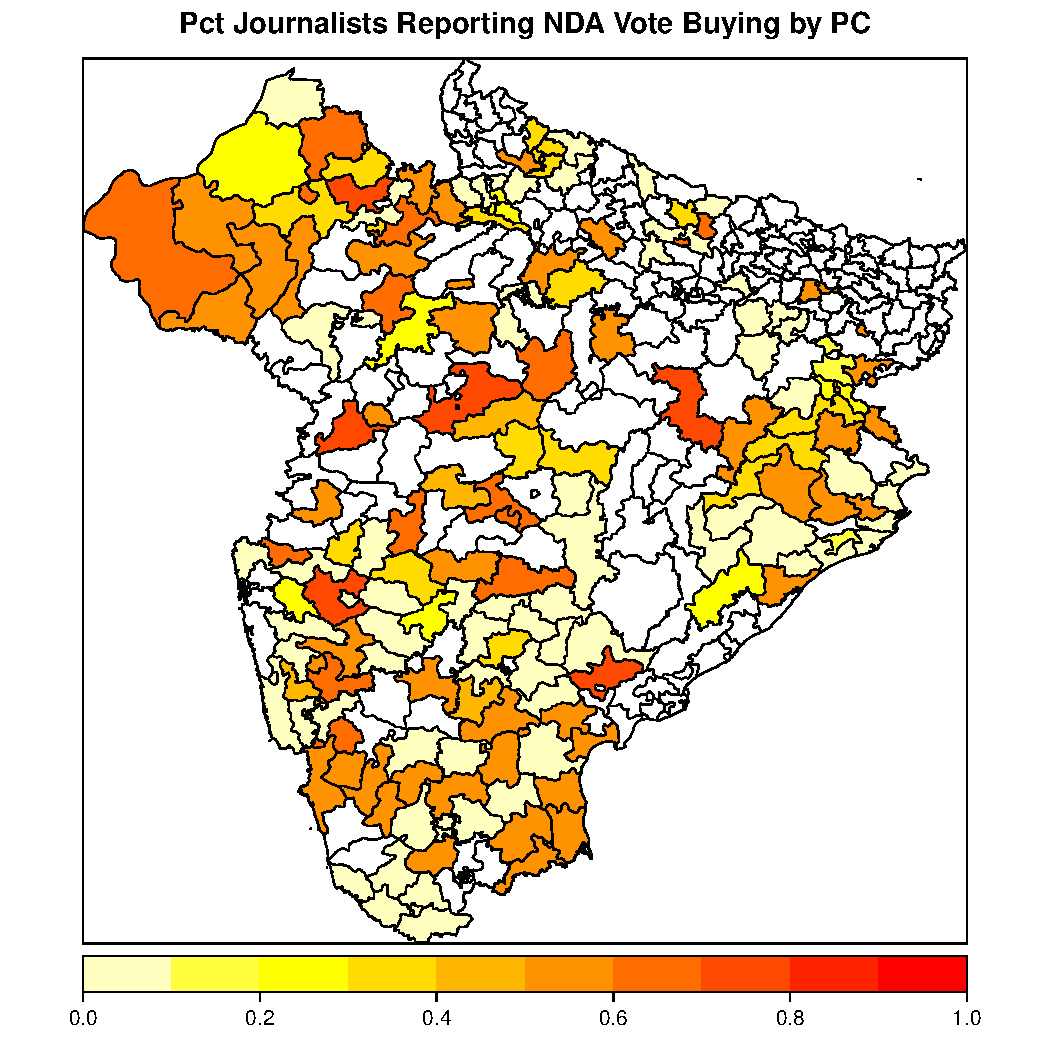
\includegraphics[width=.6\textwidth]{../Figures/nda_vb_map}
\end{figure}

\end{frame}



\begin{frame}
\frametitle{What does it mean to be a vote buying party?}

\begin{figure}
\centering
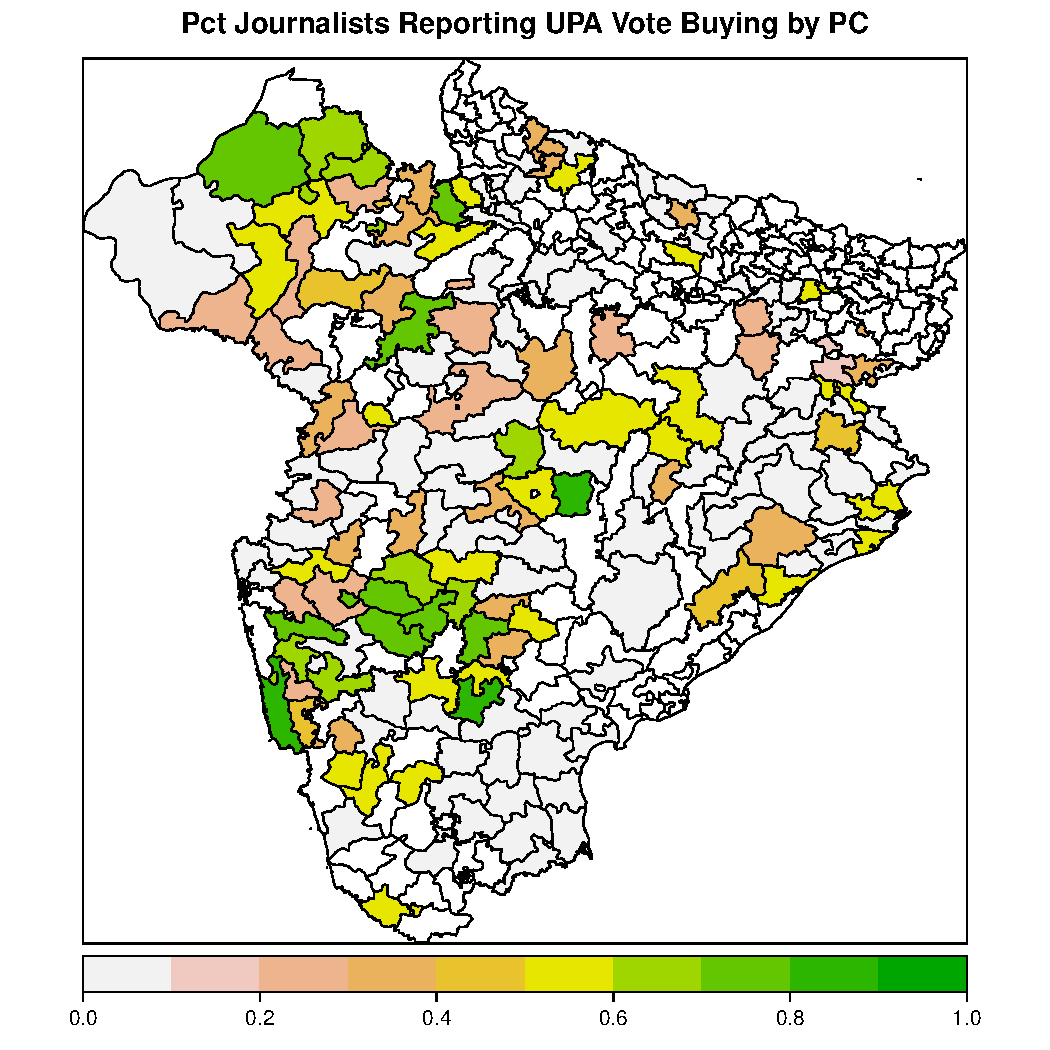
\includegraphics[width=.6\textwidth]{../Figures/upa_vb_map}
\end{figure}

\end{frame}



\begin{frame}
\frametitle{What does it mean to be a vote buying party?}

\begin{figure}
\centering
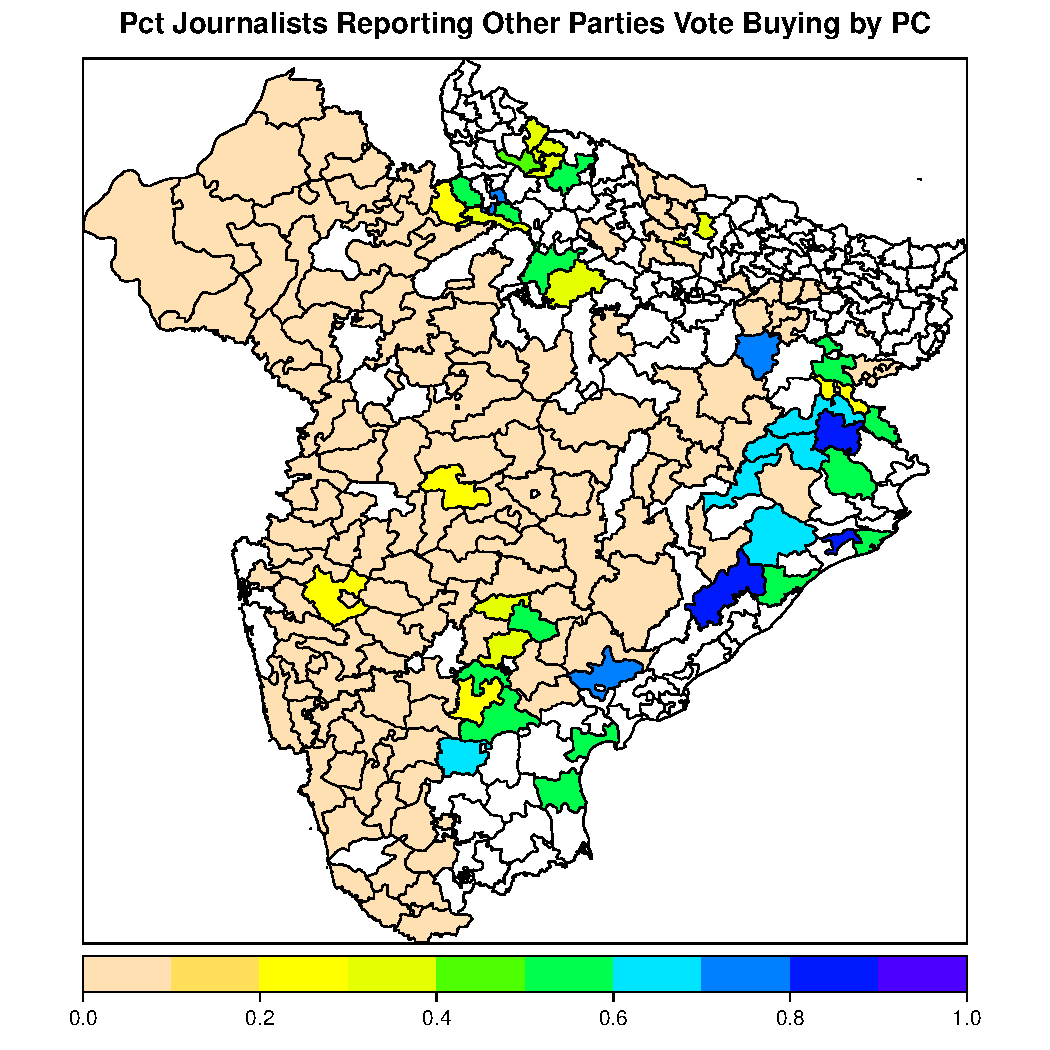
\includegraphics[width=.6\textwidth]{../Figures/oth_vb_map}
\end{figure}

\end{frame}




\begin{frame}
\frametitle{What does it mean to be a vote buying party?}

\begin{figure}
\centering
\includegraphics<1>[width=.6\textwidth]{../Figures/new_vb_defn_0}
\includegraphics<2>[width=.6\textwidth]{../Figures/new_vb_defn_1}
\includegraphics<3>[width=.6\textwidth]{../Figures/new_vb_defn_2}
\includegraphics<4>[width=.6\textwidth]{../Figures/new_vb_defn_3}
\includegraphics<5>[width=.6\textwidth]{../Figures/new_vb_defn_4}
\includegraphics<6>[width=.6\textwidth]{../Figures/new_vb_defn_5}
\includegraphics<7>[width=.6\textwidth]{../Figures/new_vb_defn_6}
\includegraphics<8>[width=.6\textwidth]{../Figures/new_vb_defn_7}
\includegraphics<9>[width=.6\textwidth]{../Figures/new_vb_defn_8}
\includegraphics<10>[width=.6\textwidth]{../Figures/new_vb_defn_9}
\end{figure}

\end{frame}



\begin{frame}
\frametitle{Robustness to the definition of vote buying party}

\begin{figure}
\centering
\includegraphics[width=.6\textwidth]{../Figures/coef_journo_defn}
\end{figure}

\end{frame}



\begin{frame}
\frametitle{Robustness to the definition of vote buying party}
\begin{figure}
\centering
\includegraphics[width=.6\textwidth]{../Figures/p_journo_defn}
\end{figure}
\end{frame}


\begin{frame}
\frametitle{Heterogeneous effects: Urban}
\begin{columns}[T] % align columns
\begin{column}{.48\textwidth}
\scalebox{.9}{
\vbox{%
\vspace{-10pt}
\begin{table}
Dummy: More than 90\% Rural\\
% latex table generated in R 3.2.2 by xtable 1.7-4 package
% Tue Oct 27 17:38:57 2015
\begin{tabular}{rlll}
  \hline
 & ATE & SE & p \\ 
  \hline
Treat & -4.68 & 3.6 & 0.1 \\ 
  Rural $>$90 pc & 1.69 & 2.55 & 0.25 \\ 
  Treat:Rural90 & -3.16 & 3.83 & 0.2 \\ 
  R squared & 0.44 &  &  \\ 
   \hline
\end{tabular}

 
\bigskip
Continuous Rural\\
% latex table generated in R 3.2.2 by xtable 1.7-4 package
% Tue Oct 27 17:38:57 2015
\begin{tabular}{rlll}
  \hline
 & ATE & SE & p \\ 
  \hline
Treat & 1.79 & 6.79 & 0.4 \\ 
  Rural pc & -0.01 & 0.05 & 0.45 \\ 
  Treat:Rural pc & -0.1 & 0.06 & 0.06 \\ 
  R squared & 0.44 &  &  \\ 
   \hline
\end{tabular}


\end{table}}}
\end{column}%
\hfill%
\begin{column}{.48\textwidth}
\vspace{-10pt}
\includegraphics[scale=.45]{../Figures/histrurpc.pdf}
\end{column}%
\end{columns}
\end{frame}



\begin{frame}
\frametitle{Heterogeneous effects: Minority voters}
\begin{columns}[T] % align columns
\begin{column}{.48\textwidth}
\scalebox{.9}{
\vbox{%
\vspace{-10pt}
\begin{table}
Dummy: $>$50\% SC/ST \\
% latex table generated in R 3.2.2 by xtable 1.7-4 package
% Tue Oct 27 17:43:32 2015
\begin{tabular}{rlll}
  \hline
 & ATE & SE & p \\ 
  \hline
Treat & -6 & 4.4 & 0.09 \\ 
  SC/ST $>$50 pc & -4.88 & 3.66 & 0.09 \\ 
  Treat:SC/ST50 & 1.87 & 5.06 & 0.36 \\ 
  R squared & 0.44 &  &  \\ 
   \hline
\end{tabular}

 
\bigskip
Continuous SC/ST\\
% latex table generated in R 3.2.2 by xtable 1.7-4 package
% Tue Oct 27 19:22:06 2015
\begin{tabular}{rlll}
  \hline
 & Coef. & SE & p \\ 
  \hline
Treat & -6.03 & 6.36 & 0.17 \\ 
  ST/SC pc & -0.06 & 0.09 & 0.26 \\ 
  Treat:SC/ST pc & 0.01 & 0.11 & 0.48 \\ 
  R squared & 0.44 &  &  \\ 
   \hline
\end{tabular}


\end{table}}}
\end{column}%
\hfill%
\begin{column}{.48\textwidth}
\vspace{-10pt}
\includegraphics[scale=.45]{../Figures/histscstpc.pdf}
\end{column}%
\end{columns}
\end{frame}


\begin{frame}
\frametitle{Heterogeneous effects: Date of election}
\scalebox{.8}{
\vbox{%
\vspace{-10pt}
\begin{table}
\caption{Elec Date by State}
% latex table generated in R 3.2.2 by xtable 1.7-4 package
% Wed Oct 28 13:55:04 2015
\begin{tabular}{rrrrrr}
  \hline
 & Andhra  & Bihar & Chattisgarh & Jharkhand & Karnataka  \\ 
 &  Pradesh &  &  &  &  \\ 
  \hline
2014-04-10 &   0 &   6 &   0 &   2 &   0 &  \\ 
  2014-04-17 &   0 &   8 &   0 &  30 &  75 & \\ 
  2014-04-24 &   0 &   0 &  42 &   0 &   0 &  \\ 
  2014-04-30 &  63 &   0 &   0 &   0 &   0 &  \\ 
  2014-05-07 &  50 &   0 &   0 &   0 &   0 &  \\ 
  2014-05-12 &   0 &   0 &   0 &   0 &   0 &  \\ 
   \hline
\end{tabular}
\medskip
\begin{tabular}{rrrrrr}
  \hline
 & Madhya  & Maharashtra & Orissa & Rajasthan & Uttar  \\ 
 &  Pradesh &  &  &  &  Pradesh \\ 
  \hline
2014-04-10 &  17 &  19 &  30 &   0 &   0 \\ 
  2014-04-17 &   10 &  45 &  19 &  64 &  24 \\ 
  2014-04-24 &   18 &  34 &   0 &  32 &   4 \\ 
  2014-04-30 &    0 &   0 &   0 &   0 &   5 \\ 
  2014-05-07 &    0 &   0 &   0 &   0 &  30 \\ 
  2014-05-12 &   0 &   0 &   0 &   0 &   1 \\ 
   \hline
\end{tabular}


\end{table}}}
\end{frame}



\begin{frame}
\frametitle{Heterogeneous effects: Date of election}
\begin{columns}[T] % align columns
\begin{column}{.55\textwidth}
\scalebox{.6}{
\vbox{%
\vspace{-40pt}

% Table created by stargazer v.5.2 by Marek Hlavac, Harvard University. E-mail: hlavac at fas.harvard.edu
% Date and time: Wed, Oct 28, 2015 - 12:49:00
\begin{table}[!htbp] \centering 
\begin{tabular}{@{\extracolsep{5pt}}lc} 
\\[-1.8ex]\hline 
\hline \\[-1.8ex] 
 & \multicolumn{1}{c}{\textit{Dependent variable:}} \\ 
\cline{2-2} 
\\[-1.8ex] & Vote Share VB 2014 \\ 
\hline \\[-1.8ex] 
 Treat & $-$17.979$^{***}$ (3.543) \\ 
  Poll 2014-04-17 & $-$3.271 (2.818) \\ 
  Poll 2014-04-24 & 0.678 (3.120) \\ 
  Poll 2014-04-30 & $-$15.522$^{***}$ (3.316) \\ 
  Poll 2014-05-07 & 32.088$^{***}$ (3.730) \\ 
  Vote Share VB 2009 & 0.634$^{***}$ (0.025) \\ 
  Num Radio 1 & 4.927 (15.262) \\ 
  Num Radio 2 & 5.406 (15.391) \\ 
  Treat:Poll 2014-04-17 & 17.296$^{***}$ (4.003) \\ 
  Treat:Poll 2014-04-24 & 12.344$^{***}$ (4.445) \\ 
  Treat:Poll 2014-04-30 & 22.415$^{***}$ (5.438) \\ 
  Treat:Poll 2014-05-07 & $-$13.280$^{***}$ (4.940) \\ 
  Constant & 26.732$^{*}$ (15.507) \\ 
 \hline \\[-1.8ex] 
Observations & 627 \\ 
R$^{2}$ & 0.590 \\ 
Adjusted R$^{2}$ & 0.582 \\ 
Residual Std. Error & 15.136 (df = 614) \\ 
F Statistic & 73.514$^{***}$ (df = 12; 614) \\ 
\hline 
\hline \\[-1.8ex] 
\textit{Note:}  & \multicolumn{1}{r}{$^{*}$p$<$0.1; $^{**}$p$<$0.05; $^{***}$p$<$0.01} \\ 
 & \multicolumn{1}{r}{Omitted Date 2014-04-10, Excludes 2014-05-12} \\ 
\end{tabular} 
\end{table} 
 }}
\end{column}%
\hfill%
\begin{column}{.35\textwidth}
\scalebox{.7}{
\vbox{%
\vspace{-5pt}
\begin{table}
\caption{Treatment by Date}
% latex table generated in R 3.2.2 by xtable 1.7-4 package
% Wed Oct 28 12:48:30 2015
\begin{tabular}{rrr}
  \hline
 & C & T \\ 
  \hline
2014-04-10 &  37 &  37 \\ 
  2014-04-17 & 131 & 144 \\ 
  2014-04-24 &  65 &  65 \\ 
  2014-04-30 &  49 &  19 \\ 
  2014-05-07 &  33 &  47 \\ 
  2014-05-12 &   0 &   1 \\ 
   \hline
\end{tabular}


\end{table}}}
\end{column}%
\end{columns}

{\footnotesize \centering{ ** SEs and p-values not adjusted for station-level treatment ** }}

\end{frame}

\begin{frame}
\frametitle{Heterogeneous effects: Competitiveness of election}
\begin{columns}[T] % align columns
\begin{column}{.38\textwidth}
\scalebox{.6}{
\vbox{%
\vspace{-40pt}

% Table created by stargazer v.5.2 by Marek Hlavac, Harvard University. E-mail: hlavac at fas.harvard.edu
% Date and time: Tue, Oct 27, 2015 - 23:19:54
\begin{table}[!htbp] \centering 
  \caption{} 
  \label{} 
\begin{tabular}{@{\extracolsep{5pt}}lc} 
\\[-1.8ex]\hline 
\hline \\[-1.8ex] 
 & \multicolumn{1}{c}{\textit{Dependent variable:}} \\ 
\cline{2-2} 
\\[-1.8ex] & VB Share 2014 \\ 
\hline \\[-1.8ex] 
 Treat & $-$4.213 (3.111) \\ 
  Margin 5-10 & 2.896 (3.058) \\ 
  Margin 10-20 & $-$1.788 (3.042) \\ 
  Margin 20-30 & $-$0.441 (3.811) \\ 
  Margin 30+ & 1.873 (5.742) \\ 
  VB share 2009 & 0.557$^{***}$ (0.031) \\ 
  1 Station & 6.856 (18.436) \\ 
  2 Stations & 9.066 (18.595) \\ 
  Treat:Margin 5-10 & $-$1.423 (4.333) \\ 
  Treat:Margin 10-20 & 1.862 (4.436) \\ 
  Treat:Margin 20-30 & $-$5.958 (5.393) \\ 
  Treat:Margin 30+ & $-$5.392 (7.175) \\ 
  Constant & 27.781 (18.620) \\ 
 \hline \\[-1.8ex] 
Observations & 531 \\ 
R$^{2}$ & 0.407 \\ 
Adjusted R$^{2}$ & 0.393 \\ 
Residual Std. Error & 18.309 (df = 518) \\ 
F Statistic & 29.575$^{***}$ (df = 12; 518) \\ 
\hline 
\hline \\[-1.8ex] 
\textit{Note:}  & \multicolumn{1}{r}{$^{*}$p$<$0.1; $^{**}$p$<$0.05; $^{***}$p$<$0.01} \\ 
\end{tabular} 
\end{table} 
 }}
\end{column}%
\hfill%
\begin{column}{.58\textwidth}
\vspace{-10pt}
\includegraphics[scale=.5]{../Figures/histcomp.pdf}
\end{column}%
\end{columns}
\end{frame}


\begin{frame}
\frametitle{Heterogeneous effects: State}
\scalebox{1}{
\vbox{%
\vspace{-10pt}
\begin{table}
\caption{Treatment Status of ACs by State}
% latex table generated in R 3.2.2 by xtable 1.7-4 package
% Tue Oct 27 18:50:48 2015
\begin{tabular}{rrr}
  \hline
 & Control AC & Treated AC \\ 
  \hline
Andhra Pradesh &  82 &  31 \\ 
  Bihar &   0 &  14 \\ 
  Chattisgarh &  15 &  27 \\ 
  Jharkhand &  15 &  17 \\ 
  Karnataka &  50 &  25 \\ 
  Madhya Pradesh &  27 &  18 \\ 
  Maharashtra &  60 &  38 \\ 
  Orissa &  23 &  26 \\ 
  Rajasthan &  42 &  54 \\ 
  Uttar Pradesh &   1 &  63 \\ 
   \hline
\end{tabular}


\end{table}}}
\end{frame}

\begin{frame}
\frametitle{Heterogeneous effects: State}
\begin{columns}[T] % align columns
\begin{column}{.40\textwidth}
\scalebox{.6}{
\vbox{%
\vspace{-40pt}

% Table created by stargazer v.5.2 by Marek Hlavac, Harvard University. E-mail: hlavac at fas.harvard.edu
% Date and time: Tue, Oct 27, 2015 - 19:03:33
\begin{table}[!htbp] \centering 
  \caption{} 
  \label{} 
\begin{tabular}{@{\extracolsep{5pt}}lc} 
\\[-1.8ex]\hline 
\hline \\[-1.8ex] 
 & \multicolumn{1}{c}{\textit{Dependent variable:}} \\ 
\cline{2-2} 
\\[-1.8ex] & 2014 Vote Share \\ 
\\[-1.8ex] & Vote Buying Parties \\ 
\hline \\[-1.8ex] 
  State Bihar & $-$26.287$^{***}$ (5.571) \\ 
  State Chattisgarh & $-$5.774 (4.893) \\ 
  State Jharkhand & $-$3.946 (4.916) \\ 
  State Karnataka & $-$8.440$^{***}$ (3.115) \\ 
  State Madhya Pradesh & $-$2.123 (3.875) \\ 
  State Maharashtra & $-$4.945$^{*}$ (2.909) \\ 
  State Orissa & $-$4.407 (4.084) \\ 
  State Rajasthan & 1.235 (3.420) \\ 
  State Uttar Pradesh & $-$61.526$^{***}$ (17.276) \\ 
  Vote Share 2009 & 0.588$^{***}$ (0.030) \\ 
  Num Radio 1 & 2.224 (17.458) \\ 
  Num Radio 2 & 1.392 (17.560) \\ 
  Constant & 35.029$^{**}$ (17.569) \\ 
 \hline 
\end{tabular} 
\end{table} 
}}
\end{column}%
\hfill%
\begin{column}{.48\textwidth}
\scalebox{.6}{
\vbox{%
\vspace{-40pt}

% Table created by stargazer v.5.2 by Marek Hlavac, Harvard University. E-mail: hlavac at fas.harvard.edu
% Date and time: Tue, Oct 27, 2015 - 19:03:33
\begin{table}[!htbp] \centering 
  \caption{} 
  \label{} 
\begin{tabular}{@{\extracolsep{5pt}}lc} 
\\[-1.8ex]\hline 
 Treat & 4.353 (3.702) \\ 
  Treat:Bihar &  \\ 
  Treat:Chattisgarh & $-$9.903 (6.618) \\ 
  Treat:Jharkhand & 0.761 (7.062) \\ 
  Treat:Karnataka & $-$3.484 (5.559) \\ 
  Treat:Madhya Pradesh & $-$11.592$^{*}$ (6.357) \\ 
  Treat:Maharashtra & $-$8.632$^{*}$ (5.113) \\ 
  Treat:Orissa & $-$8.085 (6.116) \\ 
  Treat:Rajasthan & $-$14.242$^{***}$ (5.046) \\ 
  Treat:Uttar Pradesh & 43.523$^{**}$ (17.650) \\ 
  Constant & 35.029$^{**}$ (17.569) \\ 
 \hline \\[-1.8ex] 
Observations & 628 \\ 
R$^{2}$ & 0.485 \\ 
Adjusted R$^{2}$ & 0.467 \\ 
Residual Std. Error & 17.111 (df = 606) \\ 
F Statistic & 27.158$^{***}$ (df = 21; 606) \\ 
\hline 
\hline \\[-1.8ex] 
\textit{Note:}  & \multicolumn{1}{r}{$^{*}$p$<$0.1; $^{**}$p$<$0.05; $^{***}$p$<$0.01} \\ 
\end{tabular} 
\end{table} 
}}
\end{column}%
\end{columns}
\end{frame}

\begin{frame}
\frametitle{Interpretation of the results}
Common to switch parties and punish incumbents in India.\\
Among 289 comp. ACs in 2009, 179 switched parties in 2014.\\
\includegraphics[scale=.45]{../Figures/VBcomp.pdf}
\end{frame}

\begin{frame}
\frametitle{Interpretation of the results}

Are people fleeing major parties and voting for minor parties?\\
Does this change the results of elections? \\
\medskip
Next step: 
\begin{itemize}
\item Among ACs competitive in 2009, would the treatment \\have changed election outcome?\\
\item Check if winner, runner-up parties in 2014 were vote-buyers
\item Is the winner non-VB party while runner-up is VB party?
\item Check margin of victory in 2014 - smaller than ATE?
\end{itemize}
\end{frame}




\end{document}
